\documentclass[main.tex]{subfiles}
\begin{document}

\chapter{Evaluation}

In diesem kapitel werden zuvor ausgewählte algorithmen einheitlich verglichen und die resultierenden ergebnisse ausgewertet.

\section{Protocol}

% To determine the feasibility of performing real-time plane detection on relatively inexpensive hardware, we need to conduct experiments with the selected algorithms.
\begin{itemize}
    \item wie im konzept gesagt vergleichen wir algorithmen um \$FRAGE zu beantworten
    \item zunächst definieren wir, wie und woran wir die performanz der algos vergleichen
    \item da die algos verschiedene datensätze nutzen sind sie nicht direkt vergleichbar
    \item daher führen wir einheitliche vergleiche durch
    \item es gibt keinen passenden dynamischen datensatz (inkr. aufbau + punktwolke+ GT) daher machen wir zwei experimente:
    \begin{itemize}
        \item statisch: direkt ganze wolke da
        \item dynamisch: inkrementell aufbauend
    \end{itemize}
    \item schlussendlich werden wir die resultate beider experimente vergleichen und hinsichtlich der \$FRAGE auswerten
\end{itemize}


% Another important factor for comparability is the dataset, on which the experiments are conducted.
Because most publications of the selected algorithms use a different dataset during evaluation, they are not objectively comparable.
Furthermore, to the best of our knowledge, there is no dataset, that contains an incrementally growing and unordered point cloud with corresponding ground truth.

Thus, we first evaluate the algorithms on a dataset while excluding the temporal component(static dataset). We do this by performing plane detection on whole point clouds, rather than
incrementally growing ones. 

We then perform experiments, this time including the temporal component(dynamic dataset), by performing calculations at each time step and evaluating them individually.

Lastly, through comparison, as well as analysis of those different experiments, a statement will be given as to whether and how well plane detection is
possible in real-time.

For the evaluation of a given dataset, by comparing the test results with the ground truth, we took inspiration from \citeauthor{Araújo_Oliveira_2020} \cite[Section~4]{Araújo_Oliveira_2020}.


\section{Results}
This section deals with the results of the experiments. The individual results of both experiments are presented and analyzed. 

\subsection{Results 2D-3D-S Experiments}

\begin{table}[H]
    \centering
    \begin{tabular}{c|cccc}
              & Precision & Recall & F1   & Time(s) \\ \hline
        RSPD  & 0.85      & 0.89   & 0.86 & 0.90    \\
        OPS   & 0.87      & 0.70   & 0.77 & 16.75   \\
        3DKHT & 0.75      & 0.43   & 0.53 & 0.91    \\
        OBRG  & 0.77      & 0.69   & 0.72 & 44.66
    \end{tabular}
    \caption[Overall 2D-3D-S Results]{Average results of each algorithm over the 2D-3D-S dataset.}
    \label{tab:algo-acc}
\end{table}

Every algorithm performs calculations on every scene included in 2D-3D-S.
The results of each algorithm on an individual scene type are reported in Figure~\ref{fig:stanfordaccuracy} and Figure~\ref{fig:violintime}. As shown in Table~\ref{tab:algo-acc},
RSPD produces the overall best results with an average of 85\% precision, 89\% recall and an F1-score of 86\%, as well as an average of 0.9 seconds of calculation time.
The only other algorithm that achieves similar calculation times is 3D-KHT, which takes 0.91 seconds on average. Considering our definition of \textit{real-time} in Section~\ref{sec:realtime},
RSPD and 3D-KHT are able to perform plane detecion in real-time. Still, 3D-KHT produces the worst overall accuracy results with an average precision of 75\%, recall of 43\%, and an F1-score of 53\%.

With an average of about 17 seconds(OPS) and about 44 seconds(OBRG), both algorithms do not achieve real-time plane detection (see Table~\ref{tab:algo-acc}).


\begin{figure}[]
    \centering
    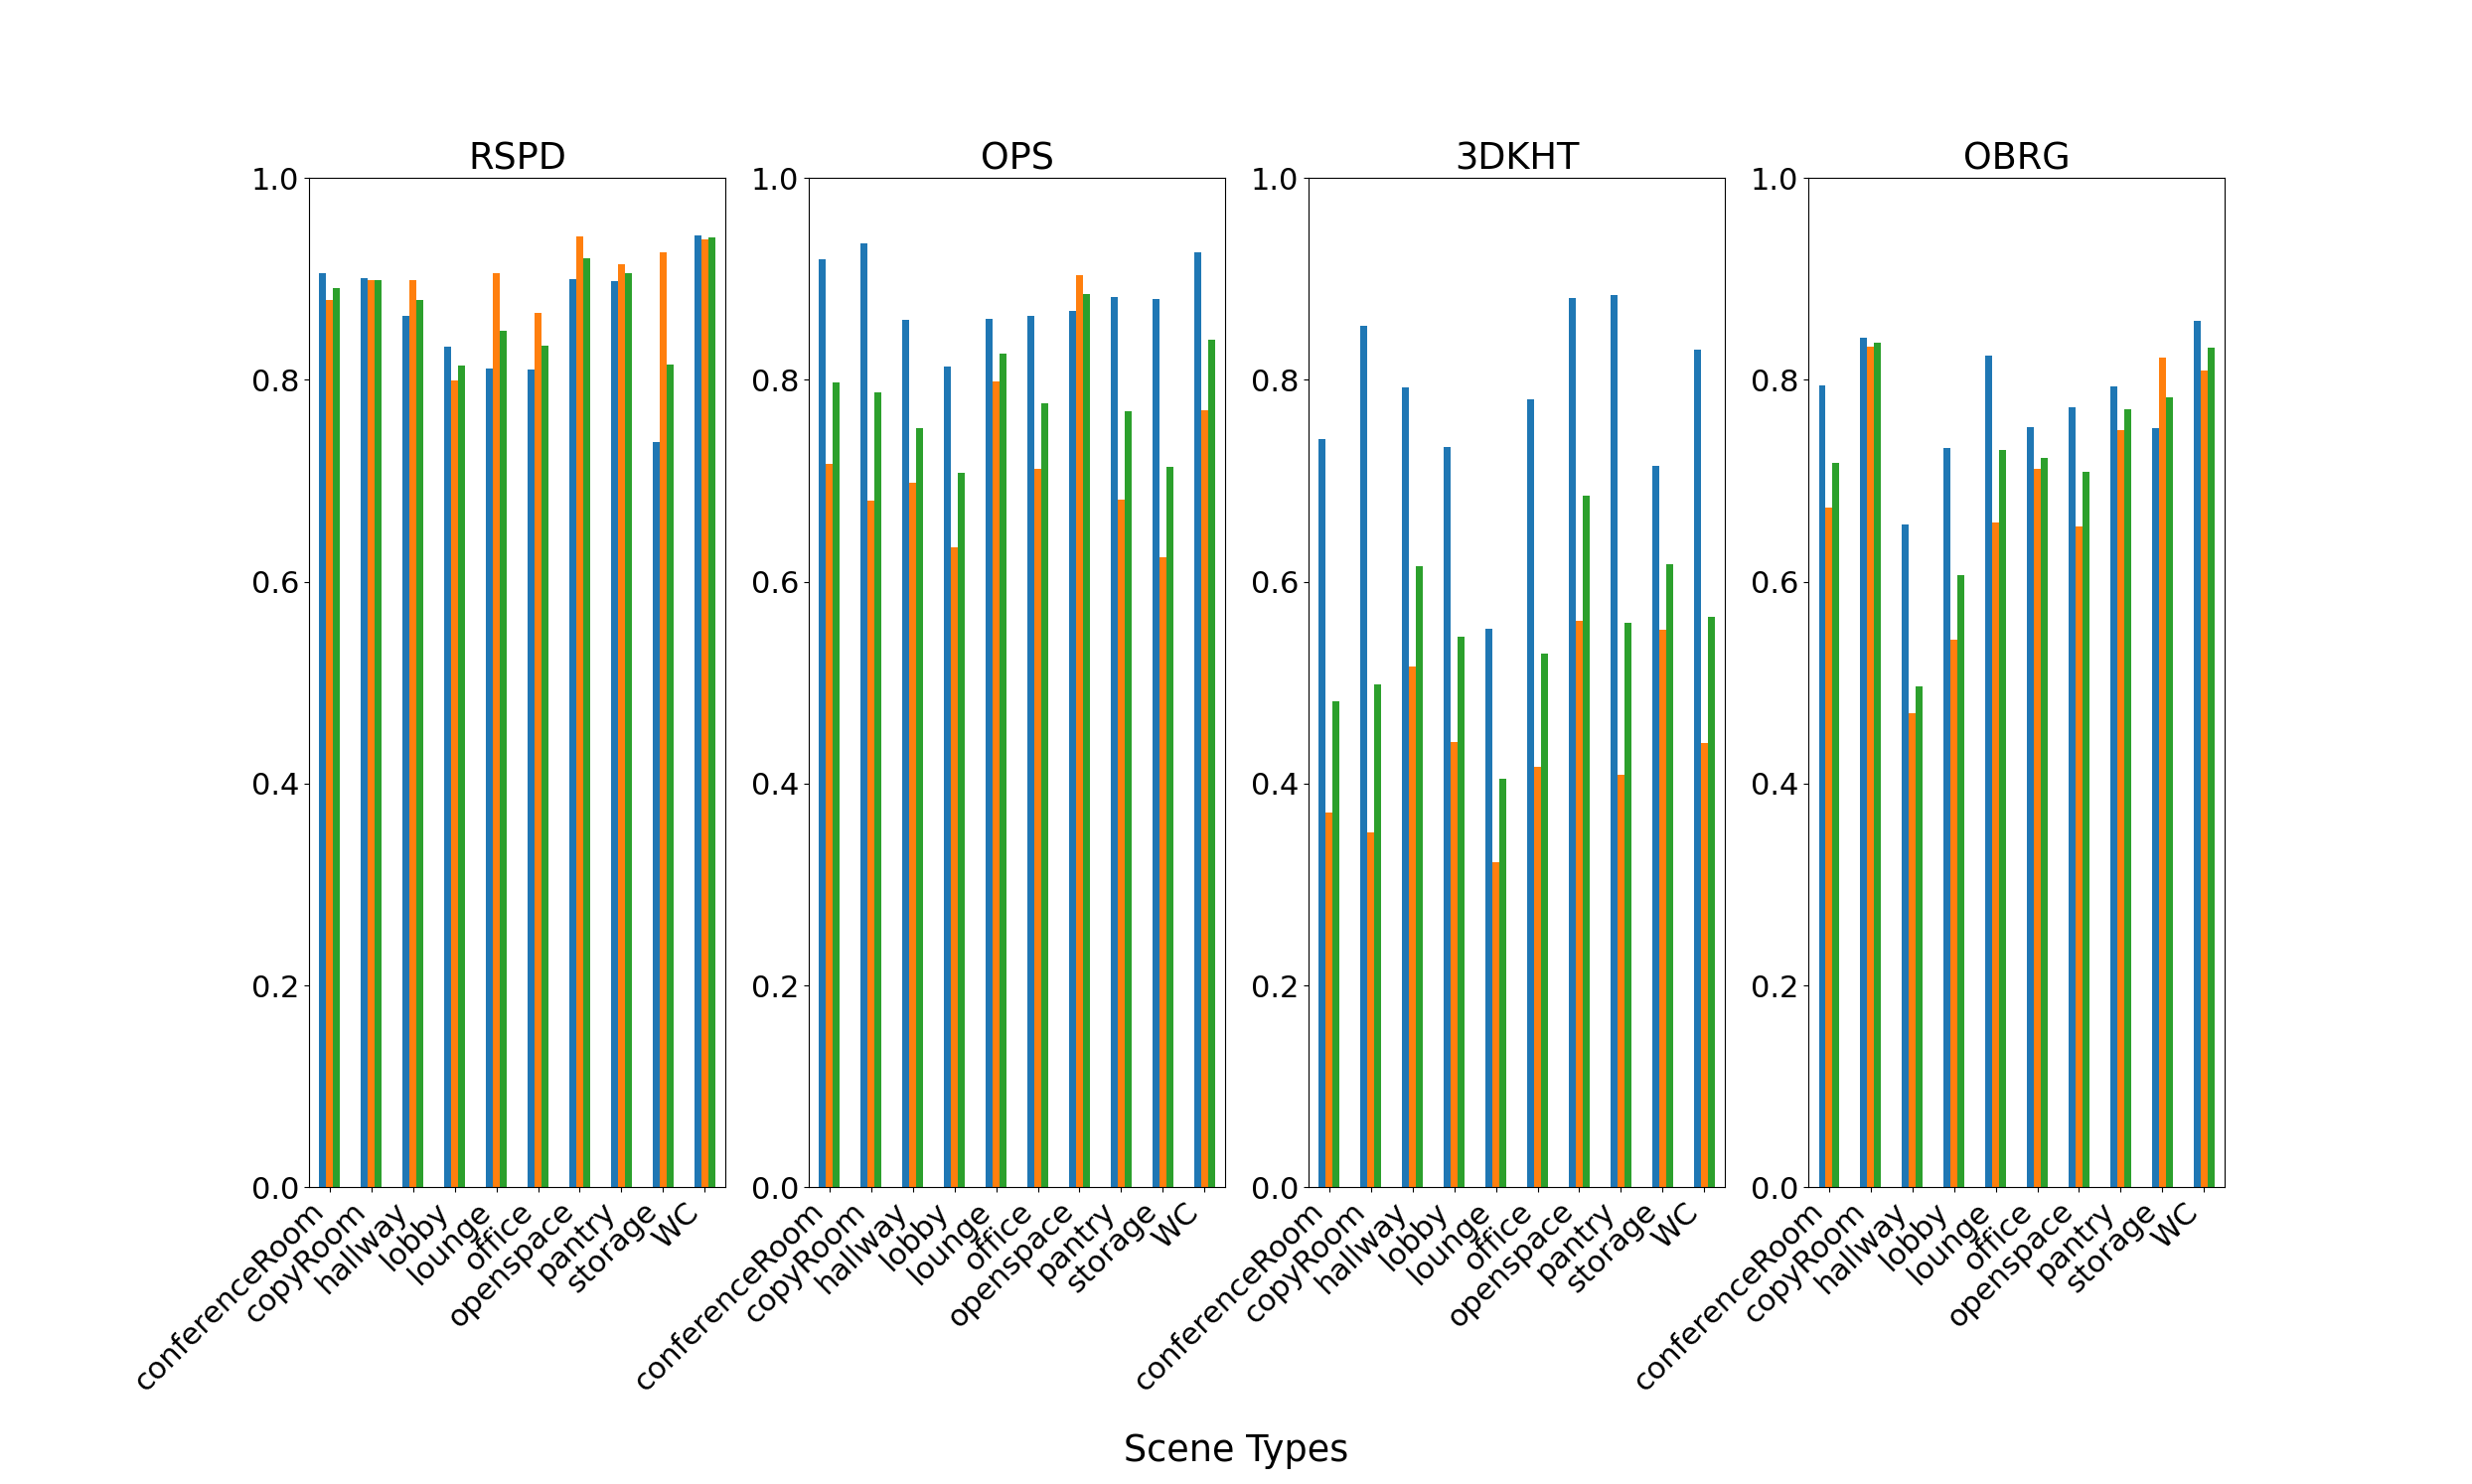
\includegraphics[width=15 cm]{images/accuracy_total.png}
    \caption[Accuracy Results 2D-3D-S]{Average Accuracy for each scene type. The Precision
        is colored blue, recall is orange and the F1-score is green.}
    \label{fig:stanfordaccuracy}
\end{figure}

\begin{figure}[]
    \centering
    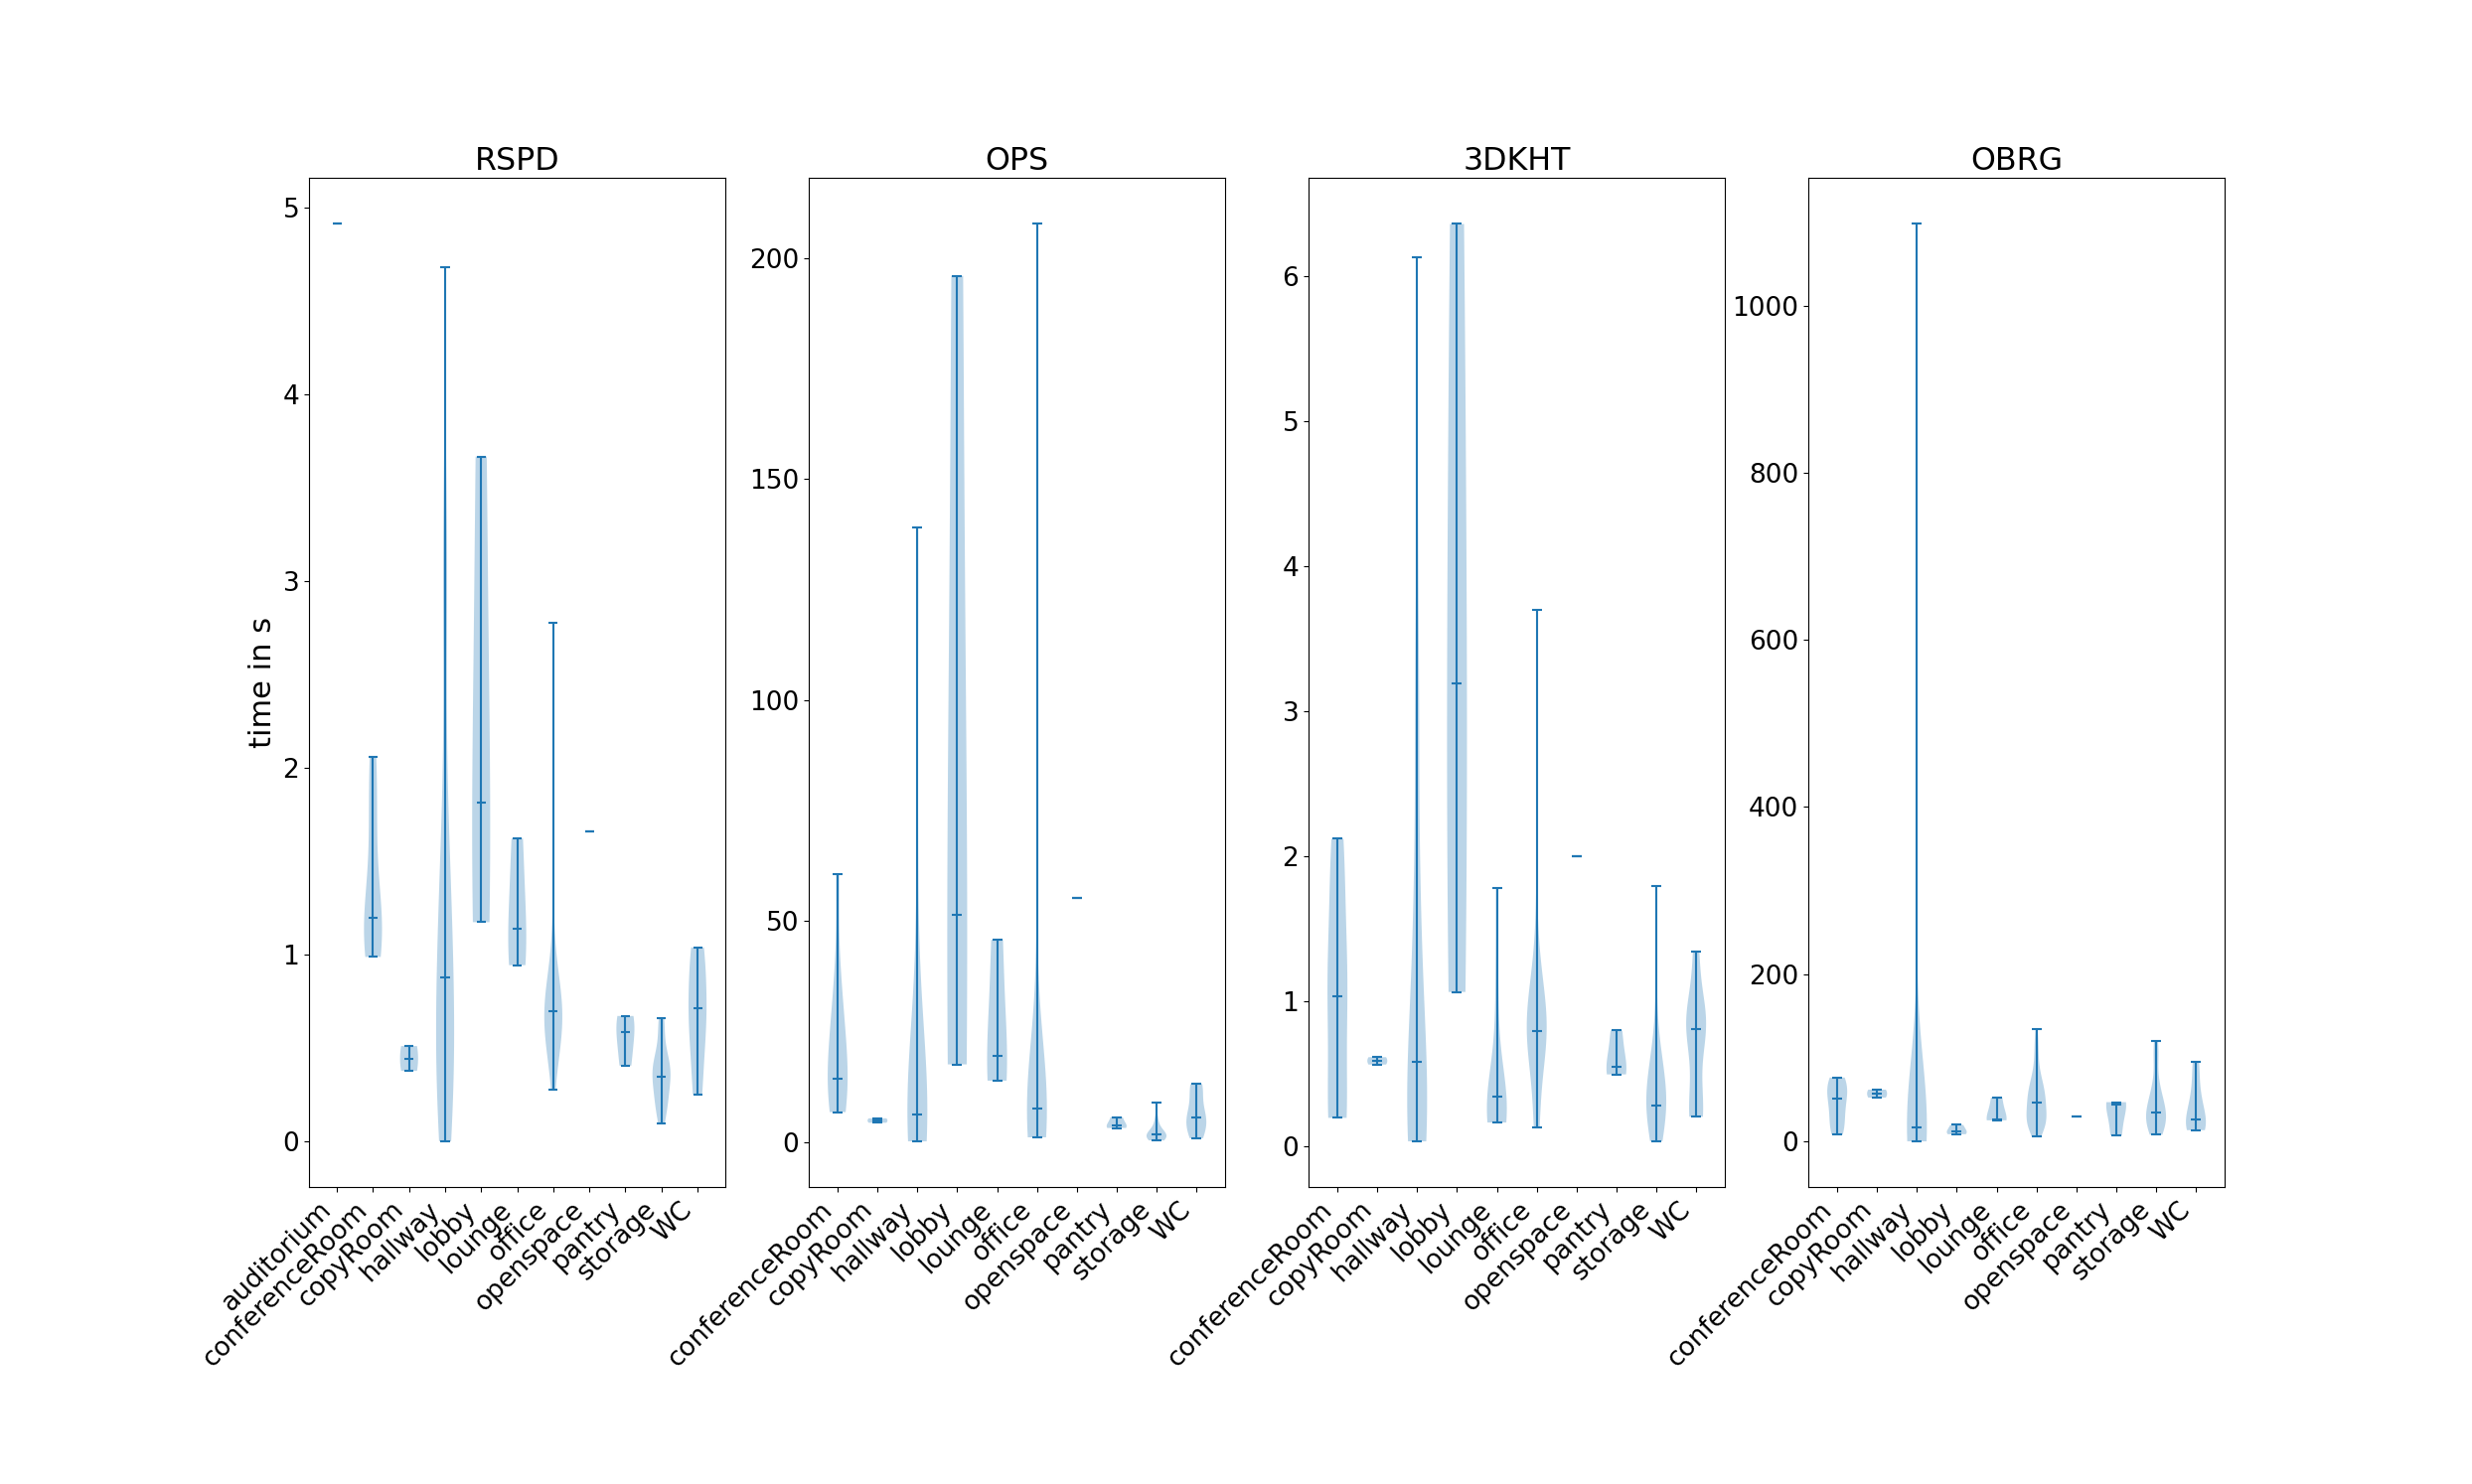
\includegraphics[width=15 cm]{images/times_violin.png}
    \caption[Time Results 2D-3D-S]{Average Time per scene type. Note, that the plots
        do not share the same y-axis.}
    \label{fig:violintime}
\end{figure}

\subsection{Results Real-Life Experiments}
\textit{So far:}

\begin{figure}[]
    \centering
    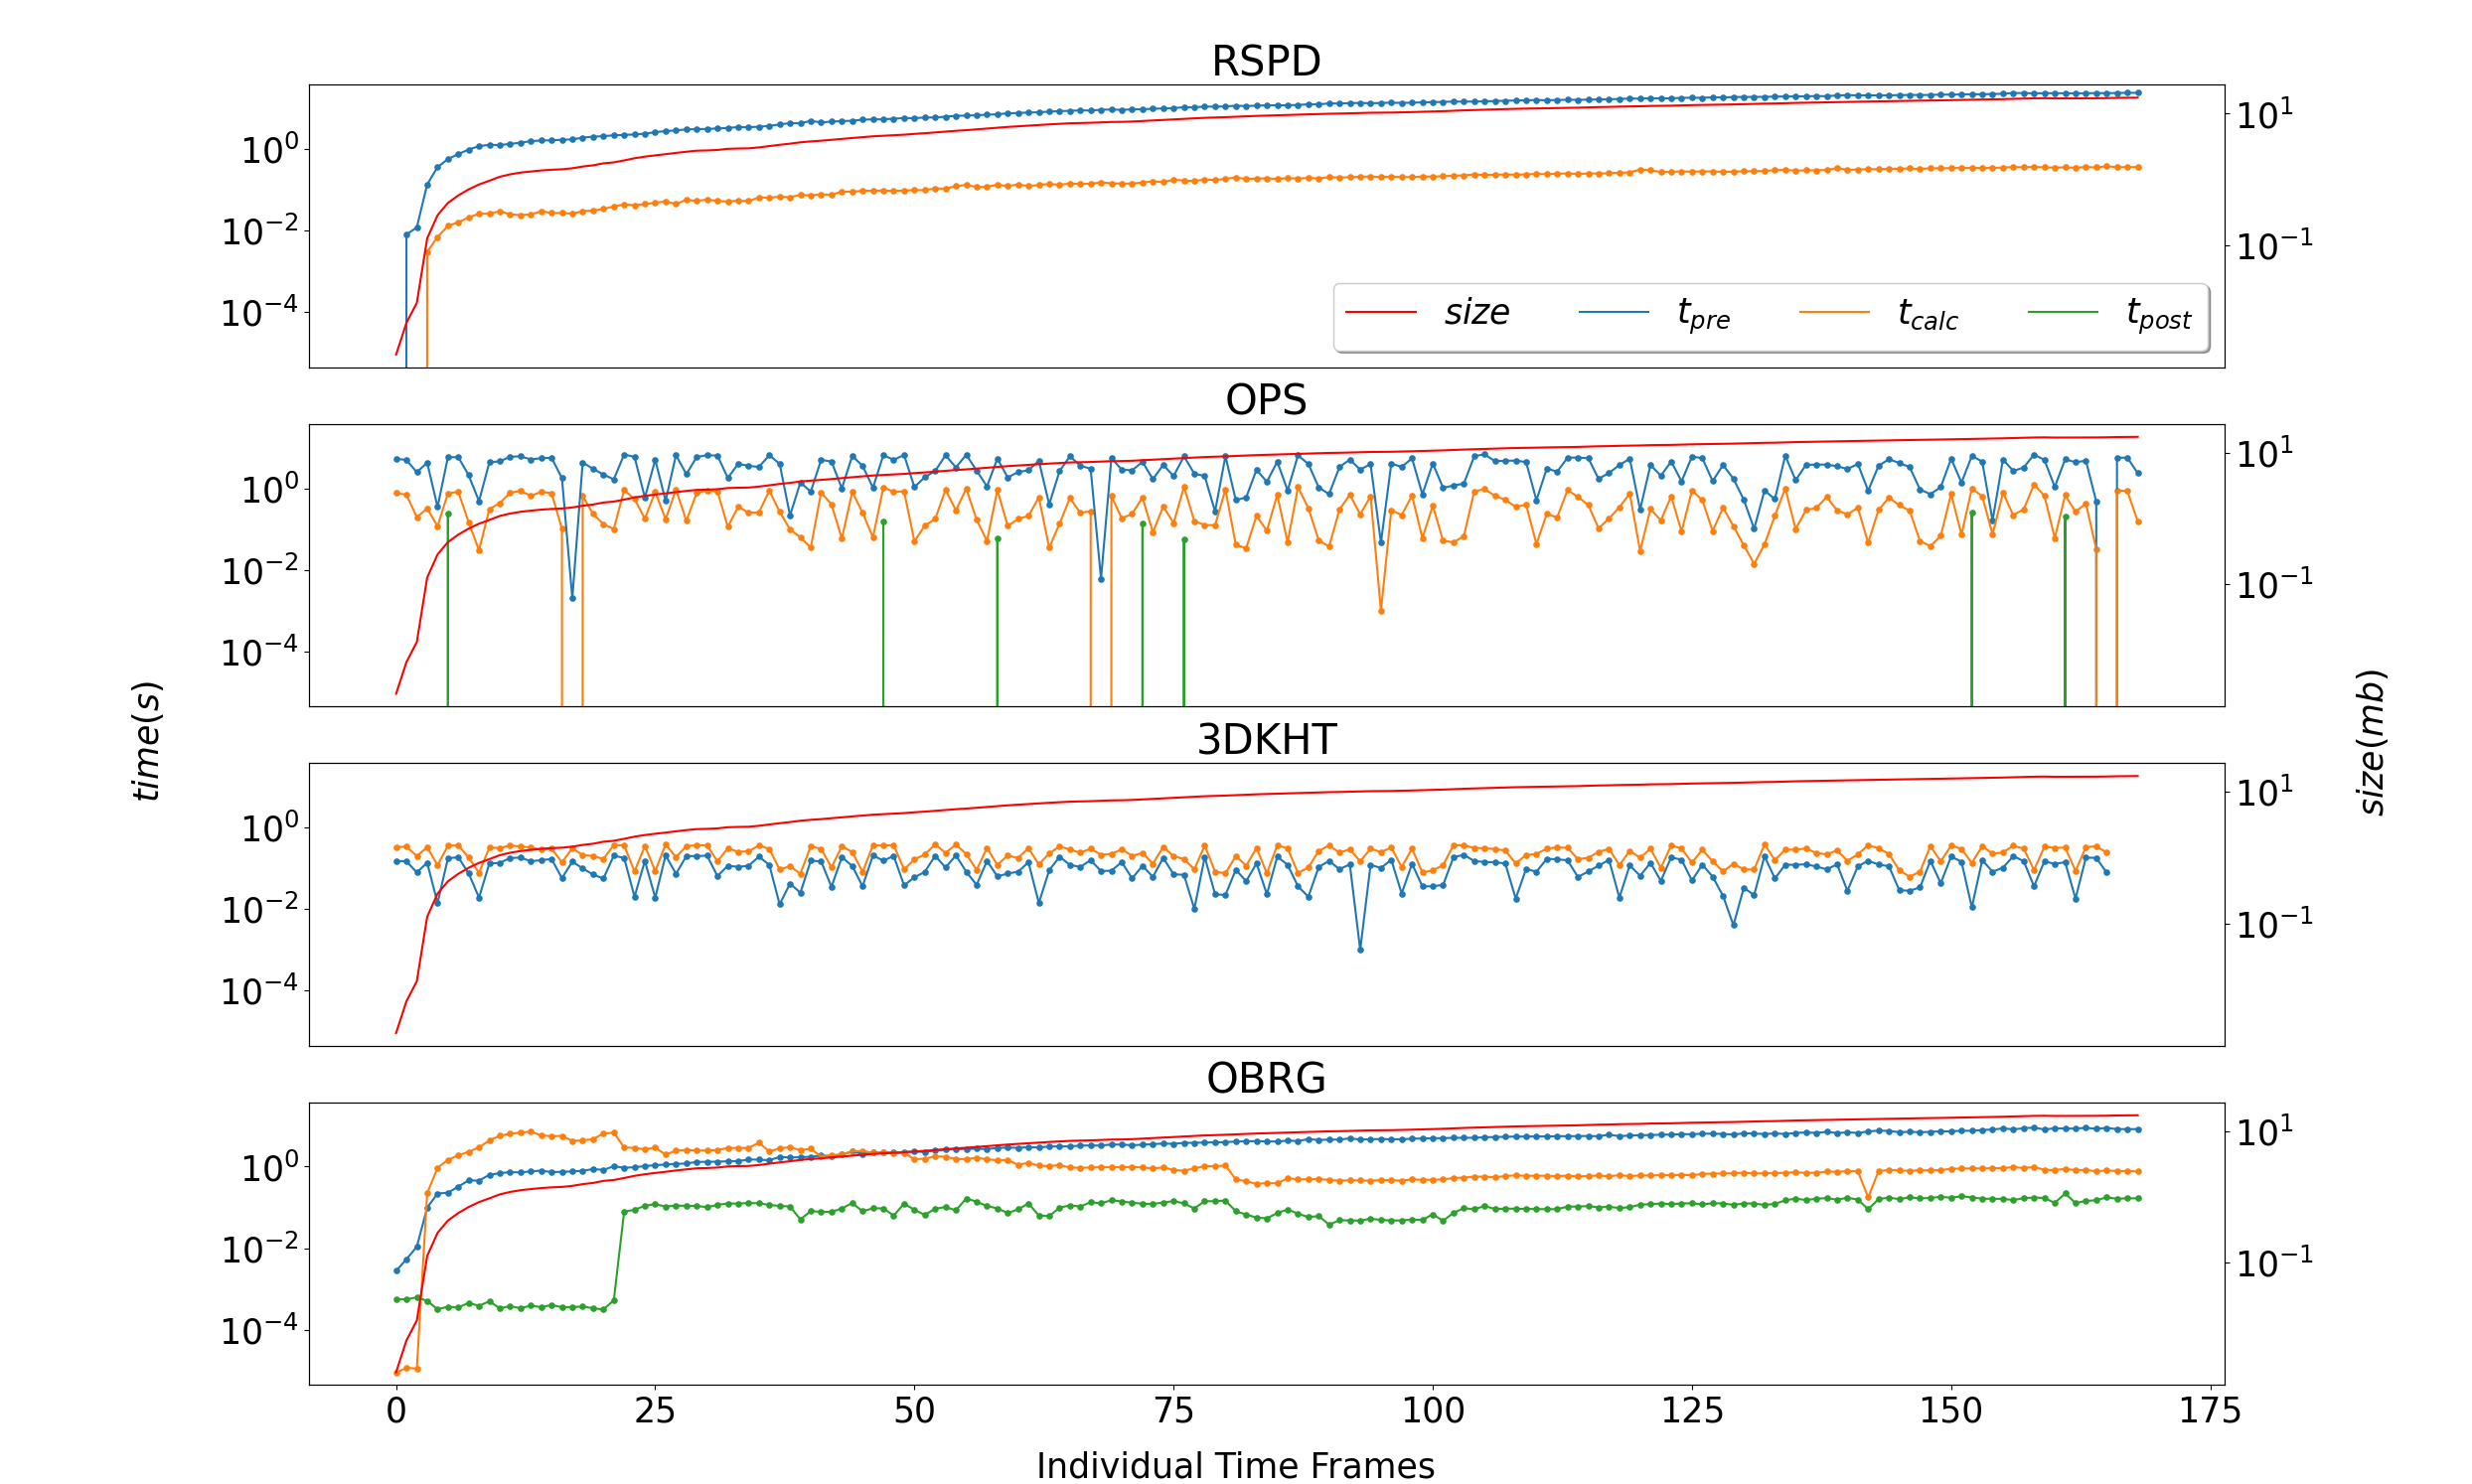
\includegraphics[width=\textwidth]{images/dyn_time-hallway.png}
    \caption[Time Results Hallway]{Calculation times(blue) of the hallway scene and cloud size(red) of each time step.}
    \label{fig:dynhallway}
\end{figure}

The calculation times of all algorithms except OBRG seem to be proportional to the size of the point cloud.
% TODO similar figure for 2D-3D-S
The quality of plane detection, however, decraeses dramatically in comparison to the Stanford Datasets. RSPD is the only dataset that
is able to detect planes. %(see Figure~\ref{fig:}). 


\subsection{Summary Results}
This section combines the preceding results of both experiments.
RSPD is the only algorithm that produces comparable results to the Stanford experiment in the dynamic experiment.
The remaining algorithms cannot reliably detect planes in an incrementally growing environment inheriting varying degrees of noise.

The reason for RSPD's dominance is likely caused by the inherent robustness against noise, as described in Section~

Die ergebnisse der beiden experimente unterscheiden sich in folgendem punkt. Dazu sei gesagt, dass die experimente folgende übereinstimmungen haben.
Das lässt sich so erklären. Alternative gründe davon könnten diese hier sein.

Ich denke RSPD ragt heraus, da hier besonders auf noise resistenz geachtet wurde. % TODO verweis auf diverse noise tests im BG


\end{document}